\chapter{SOLID}

\section{Analyse Single-Responsibility-Principle (SRP)}
\subsection{Positiv-Beispiel}
Die nachfolgende Abbildung zeigt das gekürzte UML-Diagramm der Klasse
\textit{CollectAction}. Die ist in der Schicht \textit{plugins}
angesiedelt. Sie implementiert das \textit{IAction}-Interface, welche
vom Spieler initiierte Aktionen darstellt. Die einzige Aufgabe der
\textit{CollectAction} ist es, zu prüfen, ob ein Item unter dem 
Spieler liegt und dieses aufzunehmen bzw. mit dem bisherigen Item
gleichen Typ (z.B. Rüstung) auszutauschen. Dafür bekommt es ein
\textit{Game}-Objekt übergeben, aus welchem die nötigen Informationen
gezogen und die nötigen Funktionen aufgerufen werden können.

\vspace{0.5cm}
\begin{figure}[H]
    \centering
    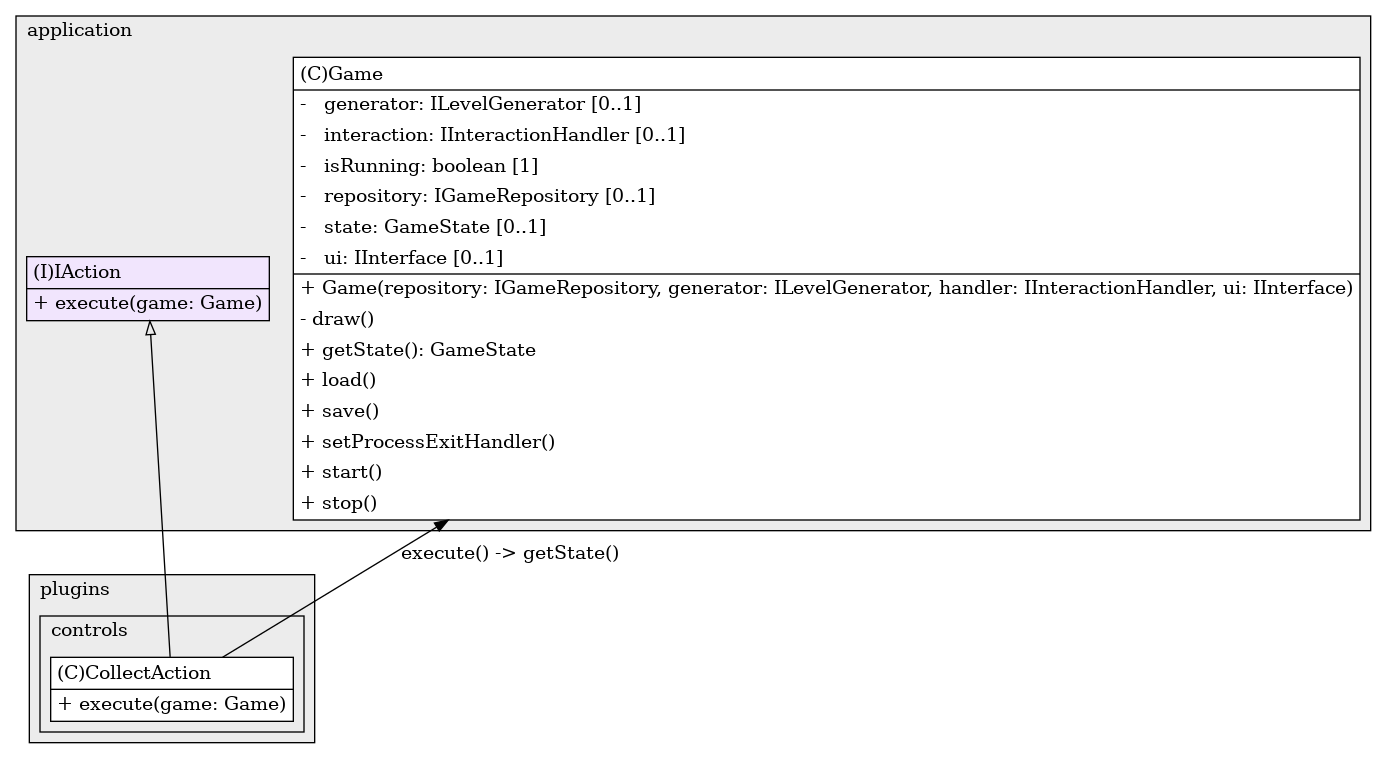
\includegraphics[width=1\linewidth]{Bilder/Visualisierung/CollectActionSimplified_structure.png}
    \caption{Analyse Single-Responsibility-Principle: Positiv}
\end{figure}

\subsection{Negativ-Beispiel}

\section{Analyse Open-Closed-Principle (OCP)}
\subsection{Positiv-Beispiel}
Die nachfolgende Abbildung zeigt das gekürzte UML-Diagramm des Interfaces
\textit{IAction}. Dieses ist in der Schicht \textit{application}
angesiedelt. Die \textit{Main}-Klasse mit ihrem \textit{Game Loop}
kennt lediglich das Aktions-Interface \textit{IAction}. Es bezieht
die Aktionen aus einem \textit{IInteractionHandler} (hier zur
Vereinfachung nicht mit dargestellt). Diese werden dann mittels
ihrer \textit{execute()}-Methode ausgeführt. 

Diese Struktur ermöglicht die Einhaltung des
\textit{Open-Closed-Principles}. Um eine neue Aktion zu implementieren,
muss lediglich eine weitere Klasse hinzugefügt werden, welche das 
\textit{IAction}-Interface implementiert. Alle anderen Implementierungen
des \textit{IAction}-Interface bleiben dabei unberührt, ebenso wie die
\textit{Main}-Klasse.

Die Verwendung dieses Schemas ist sehr sinnvoll, da vor allem in den
frühen Phasen der Spielentwicklung viele Änderungen bezüglich der
Spielerfahrung gemacht werden. Davon sind auch Aktionen und
Tasteneingaben betroffen. Mit dem \textit{IAction}-Interface lassen
sich somit schnell Änderungen mit minimalem Eingriff umsetzen. Es
müssen keine schnell unübersichtlichen \textit{switch}-Statements
benutzt werden. 

\vspace{0.2cm}
\begin{figure}[H]
    \centering
    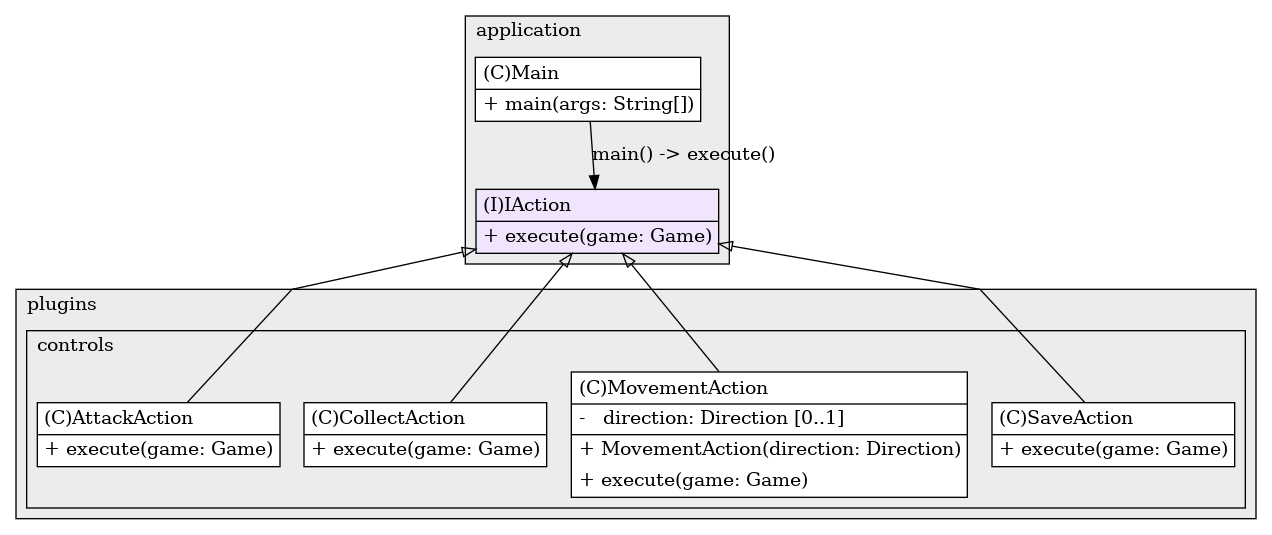
\includegraphics[width=1\linewidth]{Bilder/Visualisierung/IAction_structure.png}
    \caption{Analyse Open-Closed-Principle: Positiv}
\end{figure}

\subsection{Negativ-Beispiel}
Die nachfolgende Abbildung zeigt das UML-Diagramm der Klasse
\textit{KeyInputHandler}. Dieses ist in der Schicht \textit{plugins}
angesiedelt. Es hält eine \textit{Registry} inne, in welcher zu einigen
Tasteneingaben entsprechende Aktionen (siehe \textit{IAction}) 
hinterlegt sind. Anhand der Einträge wird dann bei einer Eingabe die
korrekte Aktion gesucht, auf eine \textit{Queue} gelegt und später im
\textit{Game Loop} ausgeführt. Die Eintragungen erfolgen im
\textit{Static Initialization Block} der Klasse. Das bedeutet, dass
die Klasse editiert werden muss, wenn neue Aktionen in das Spiel
aufgenommen und mit Tasten belegt werden. Dies widerspricht dem 
\textit{Open-Closed-Principle}.

\vspace{0.5cm}
\begin{figure}[H]
    \centering
    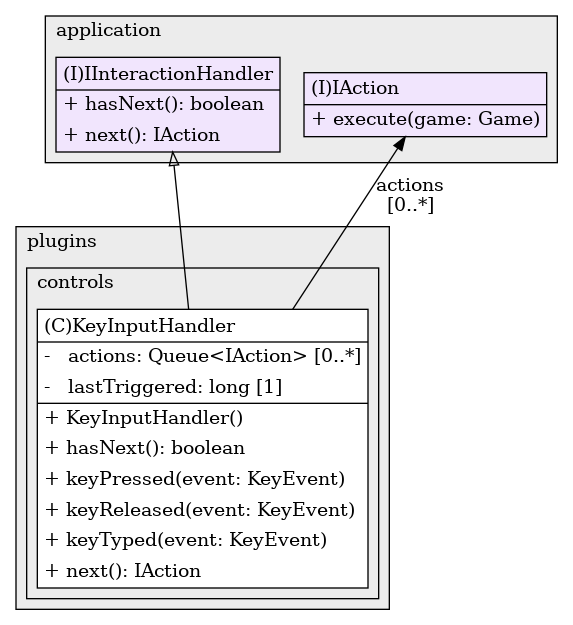
\includegraphics[width=0.5\linewidth]{Bilder/Visualisierung/KeyInputHandlerOCPViolation_structure.png}
    \caption{Analyse Open-Closed-Principle: Negativ}
\end{figure}

\section{Analyse Dependency-Inversion-Principle (DIP)}
\subsection{Positiv-Beispiel}
Die nachfolgende Abbildung zeigt das UML-Diagramm der Klasse
\textit{IGameRepository}. Dieses ist in der Schicht \textit{plugins}
angesiedelt. Wie an den Pfeilen zu sehen ist, arbeiten die Schichten
\textit{application} und \textit{plugins} über das Interface
namens \textit{IGameRepository} als Vermittler miteinander. Beide
Pfeile laufen auf das Interface zu. 

Das \textit{Dependency-Inversion-Principle} ist erfüllt, da eine
gemeinsame abstrakte Abmachung zwischen den Schichten besteht. Die
Klasse \textit{Game} hat keine Abhängigkeit zur Funktionalität der
Klasse \textit{FileGameRepository}, lediglich zu einer Abstraktion,
mit welcher Funktionalität versichert wird. Stattdessen ist die
Abhängigkeit umgekehrt (\textit{Dependency Inversion}). Die Klasse
\textit{FileGameRepository} hat eine Abhängigkeit nach innen, nämlich
zum Interface \textit{IGameRepository}. Somit lassen sich leicht
Änderungen am \textit{FileGameRepository} vornehmen oder dieser gar
durch eine ganz andere Persistenz-Methode ausgetauscht werden, ohne
dass die Klasse \textit{Game} davon direkt betroffen ist.

\enlargethispage*{2\baselineskip}
\vspace{0.5cm}
\begin{figure}[H]
    \centering
    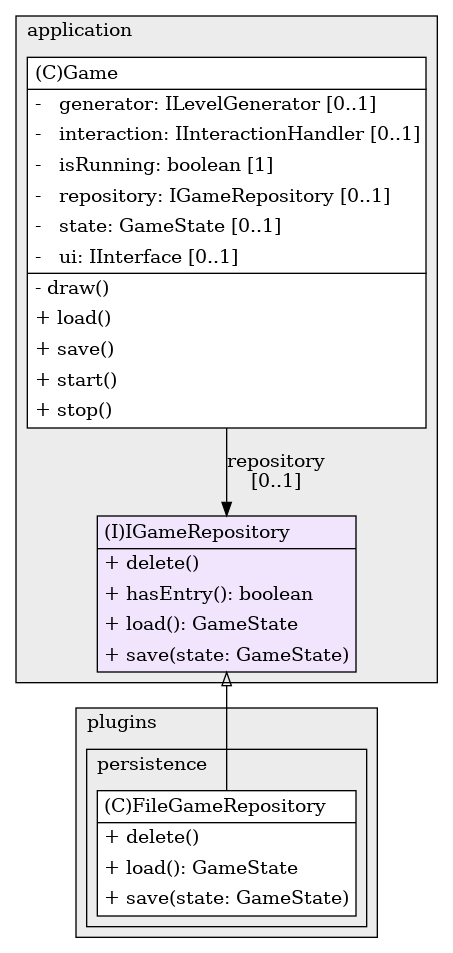
\includegraphics[width=0.3\linewidth]{Bilder/Visualisierung/IGameRepository_structure.png}
    \caption{Analyse Dependency-Inversion-Principle: Positiv}
\end{figure}

\subsection{Negativ-Beispiel}